\documentclass[a4paper,11pt]{article}
\usepackage{amsmath,amsthm,amssymb}
\usepackage{graphicx,subcaption,tikz}

\begin{document}

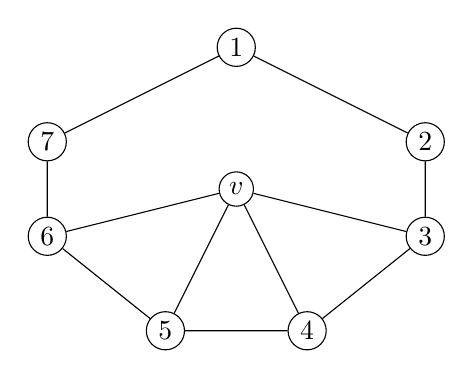
\begin{tikzpicture}[scale=0.6]
  \tikzstyle{vertex}=[draw, circle, fill=white!100, minimum width=4pt,inner sep=2pt]
  
  \node[vertex] (v1) at (0,3) {1};
  \node[vertex] (v2) at (4,1) {2};
  \node[vertex] (v3) at (4,-1) {3};
  \node[vertex] (v4) at (1.5,-3) {4};
  \node[vertex] (v5) at (-1.5,-3) {5};
  \node[vertex] (v6) at (-4,-1) {6};
  \node[vertex] (v7) at (-4,1) {7};
  \draw (v1)--(v2)--(v3)--(v4)--(v5)--(v6)--(v7)--(v1);
 
  \node[vertex] (v0) at (0,0) {$v$};
  \draw (v0)--(v3) (v0)--(v4) (v0)--(v5) (v0)--(v6);
 \end{tikzpicture}

\end{document}